\section{\ce{[Cu(N_3)_2(4-methoxypyridine)_2]_n}}
\subsection{Synthesis}
0.48 g \ce{Cu(NO_3)_2* 3 H_2O} (2 mmol), 0.26 g Na-azide (4 mmol) and 0.44 g 4-methoxy-pyridine (4 mmol) were dissolved in 50 mL distilled \ce{H_2O}. The solution was stirred for 2 hours  at 50$^\circ$C followed by a filtration of the resulting green solution. The mixture was stirred again for 55 minutes at the same temperature and then cooled down to room temperature. After 24 hours green needle-shaped crystals were obtained. Anal. Calculated for \ce{C_{12}H_{14}CuN_{8}O_{2}} (365.86 g/mol) : 39.40\% C; 3.86\% H; 30.63\% N; Found: 39.13 \% C; 3.87\% H; 30.52 \% N; IR (ATR, cm$^{-1}$): 2093 (s), 1616 (s), 1569 (m), 1512 (s), 1434 (m), 1301 (s), 1210 (s), 1062 (m), 1033 (s), 1009 (s), 822 (s), 660 (w), 602 (w), 576 (w), 533 (vs), 469 (m)


\begin{figure}[h!]
\centering
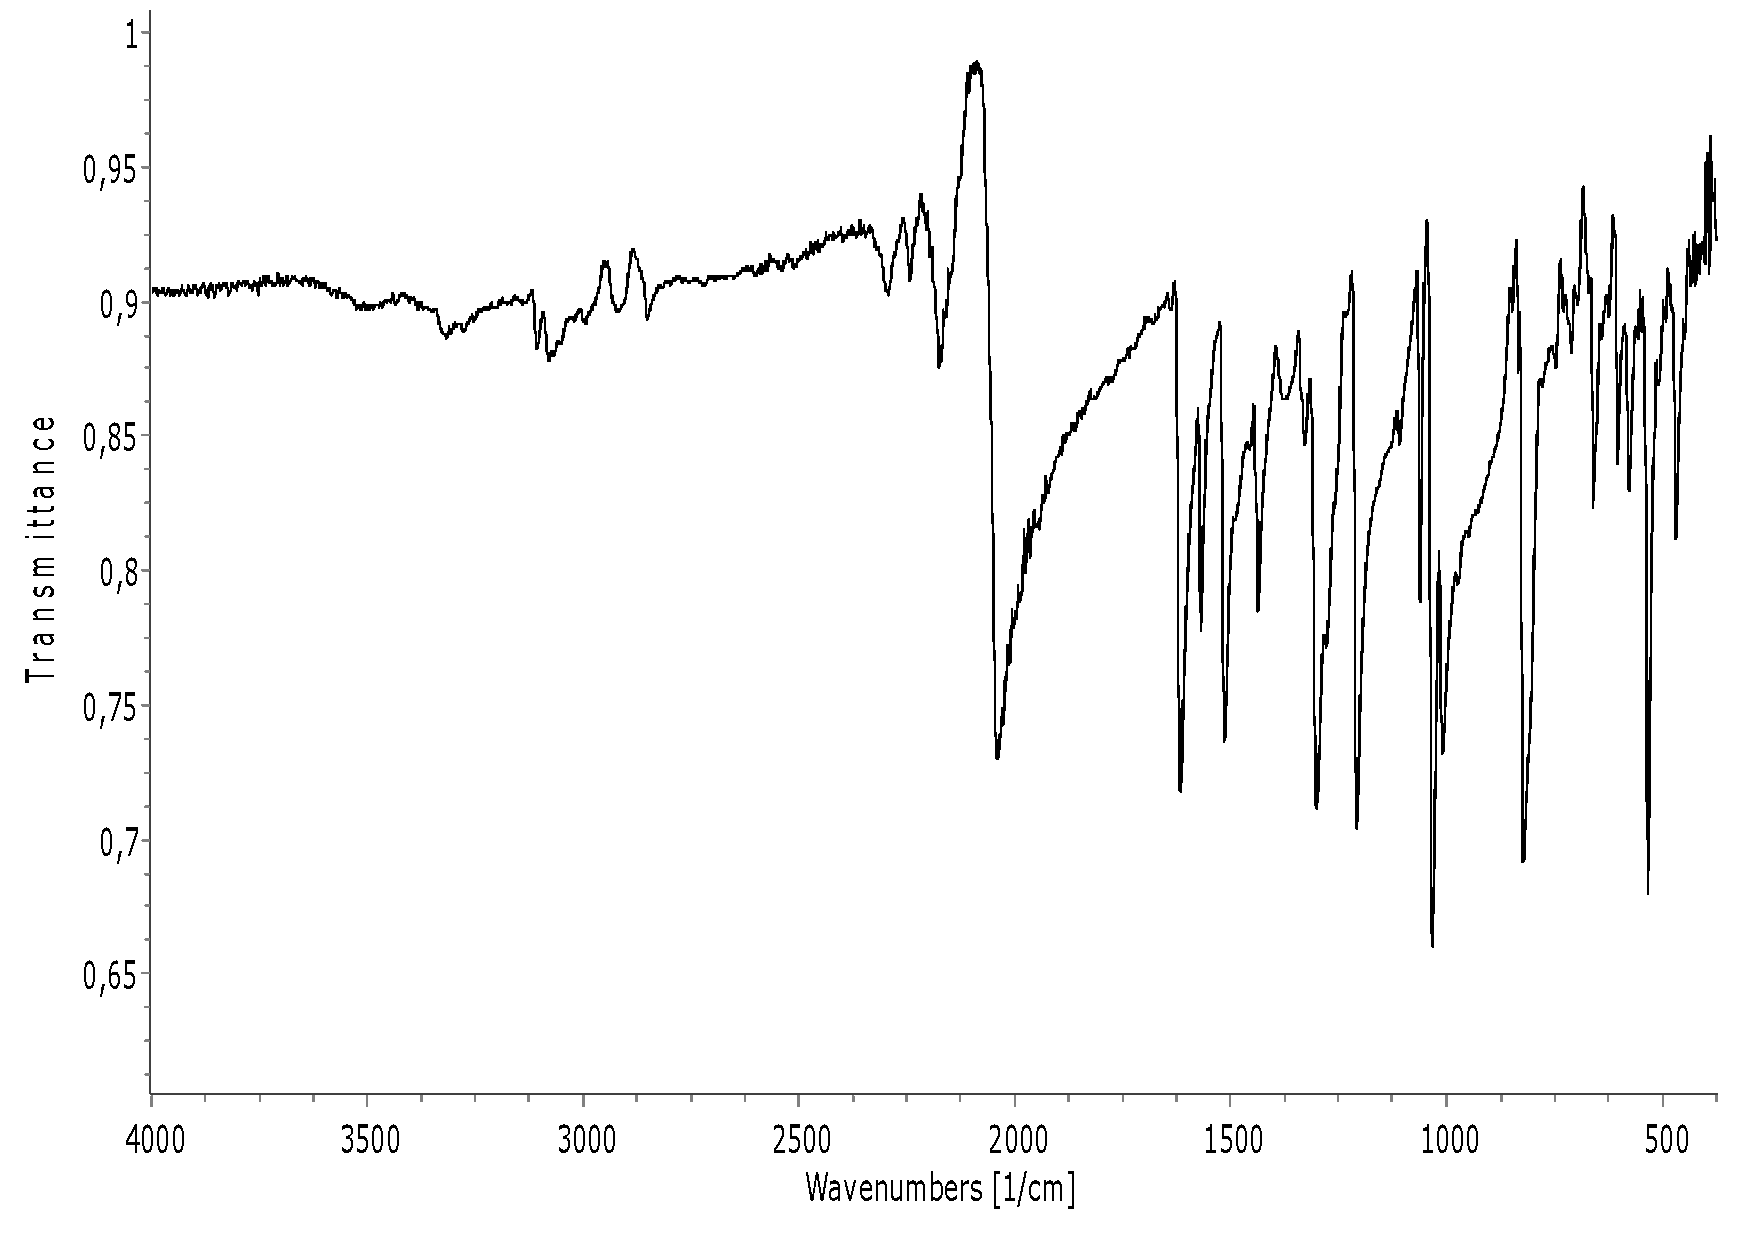
\includegraphics[width=1\textwidth]{figures/CuA4MOP-IR.pdf}
\caption{IR spectrum of \ce{[Cu(N_3)_2(4-MeOpy)_2]_n}}
\end{figure}

\subsection{Structural characterization}

A perspective view of \ce{[Cu(N_3)_2(4-MeOpy)_2]_n} is given in fig. \ref{fig:CuA4MOP_pv}, a packing view in fig. \ref{fig:CuA4MOP_packv} and selected bond parameters are summarized in table \ref{batab:CuA4MOP}. The Cu(1) metal center is located on an inversion center. It is coordinated via the pyridine N donor atom of two 4-MOP molecules in trans configuration and four N(11) atoms of azide groups. The latter act as bis-EO bridging ligands to generate polymeric chains of polyhedra along the a-axis of the triclinic unit cell. The \ce{CuN_6} chromophore may be described as axially elongated square bipyramid with longer Cu(1)-N(11b) bond distance of 2.736(4) \AA, and shorter bond distances of 2.022(4) and 2.009(3) \AA, for Cu(1)-N(11) and Cu(1)-N(1), respectively. The following bond angles are observed for the bis-EO azide bridging system: N(11)-Cu(1)-N(11c ) = 79.56(14), Cu(1)-N(11)-Cu(1c) = 100.4(2), Cu(1)-N(11)-N(12) = 121.3(3) and N(11)-N(12)-N(13) = 178.0(4)$^\circ$. The intra-chain Cu-Cu distance is 3.6846(14) and the shortest inter-chain metal-metal separation is 7.369(3) \AA.
\renewcommand{\arraystretch}{1.3}

\begin{table}[ htpb!]
\centering
\captionabove{Selected bond lengths (\AA) and angles ($^\circ$) for \ce{[Cu(N_3)_2(4-MeOpy)_2]_n}}
\begin{tabular}{|l|l|l|l|}
\hline
Cu(1)-N(1a) & 2.009(3) & Cu(1)-N(11b) & 2.736(4)\\
\hline
Cu(1)-N(11a) & 2.022(4) & N(11)-N(12) & 1.197(5)\\
\hline
N(12)-N(13) & 1.162(5) &  & \\
\hline
\hline
N(1a)-Cu(1)-N(11a) & 91.46(14) & N(11)-Cu(1)-N(11c) & 79.56(4)\\
\hline
N(1)-Cu(1)-N(1a) & 180.0 & N(11)-Cu(1)-N(11a) & 180.0\\
\hline
N(11b)-Cu(1)-N(11c) & 180.0 & N(11)-Cu(1)-N(11b) & 100.44(14)\\
\hline
Cu(1)-N(11)-N(12) & 121.3(3) & N(11)-N(12)-N(13) & 178.0(4)\\
\hline
\end{tabular}
\label{batab:CuA4MOP}
\end{table}



\begin{figure}[!htpb]
\centering
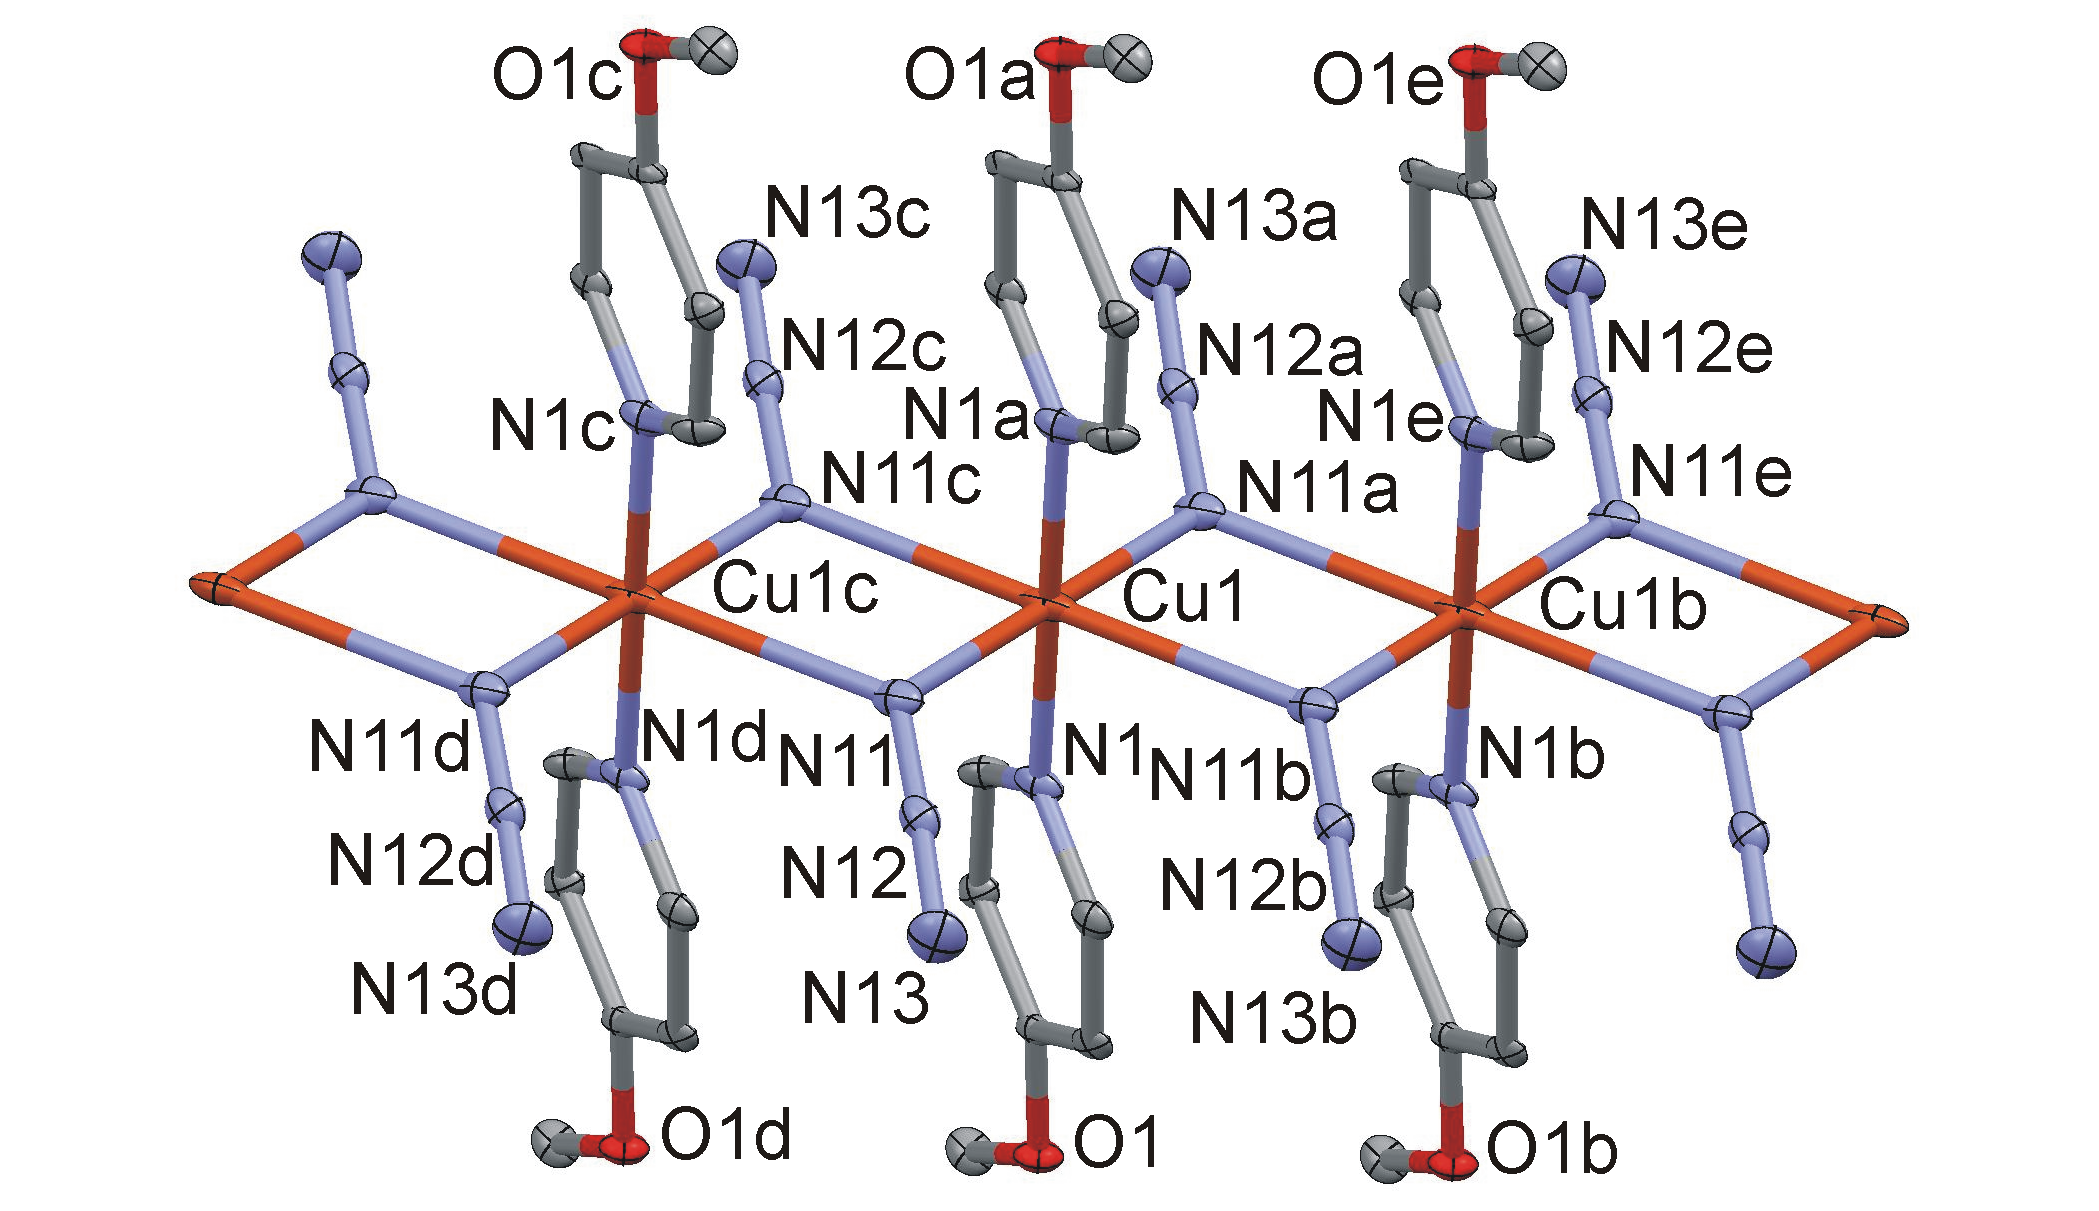
\includegraphics[width=0.95\textwidth]{figures/CuA4MOP_FIGm12.png}
\caption[Perspective view of \ce{[Cu(N_3)_2(4-MeOpy)_2]_n}]{Perspective view of a section of the polymeric chain of \ce{[Cu(N_3)_2(4-MeOpy)_2]_n} with the atom numbering scheme. Symmetry code:(a) 1-x,1-y,1-z; (b) -1+x,y,z; (c) 2-x,1-y,1-z; (d) 1+x,y,z; 
(e) –x,1-y,1-z.}
\label{fig:CuA4MOP_pv}
\vspace{\floatsep}
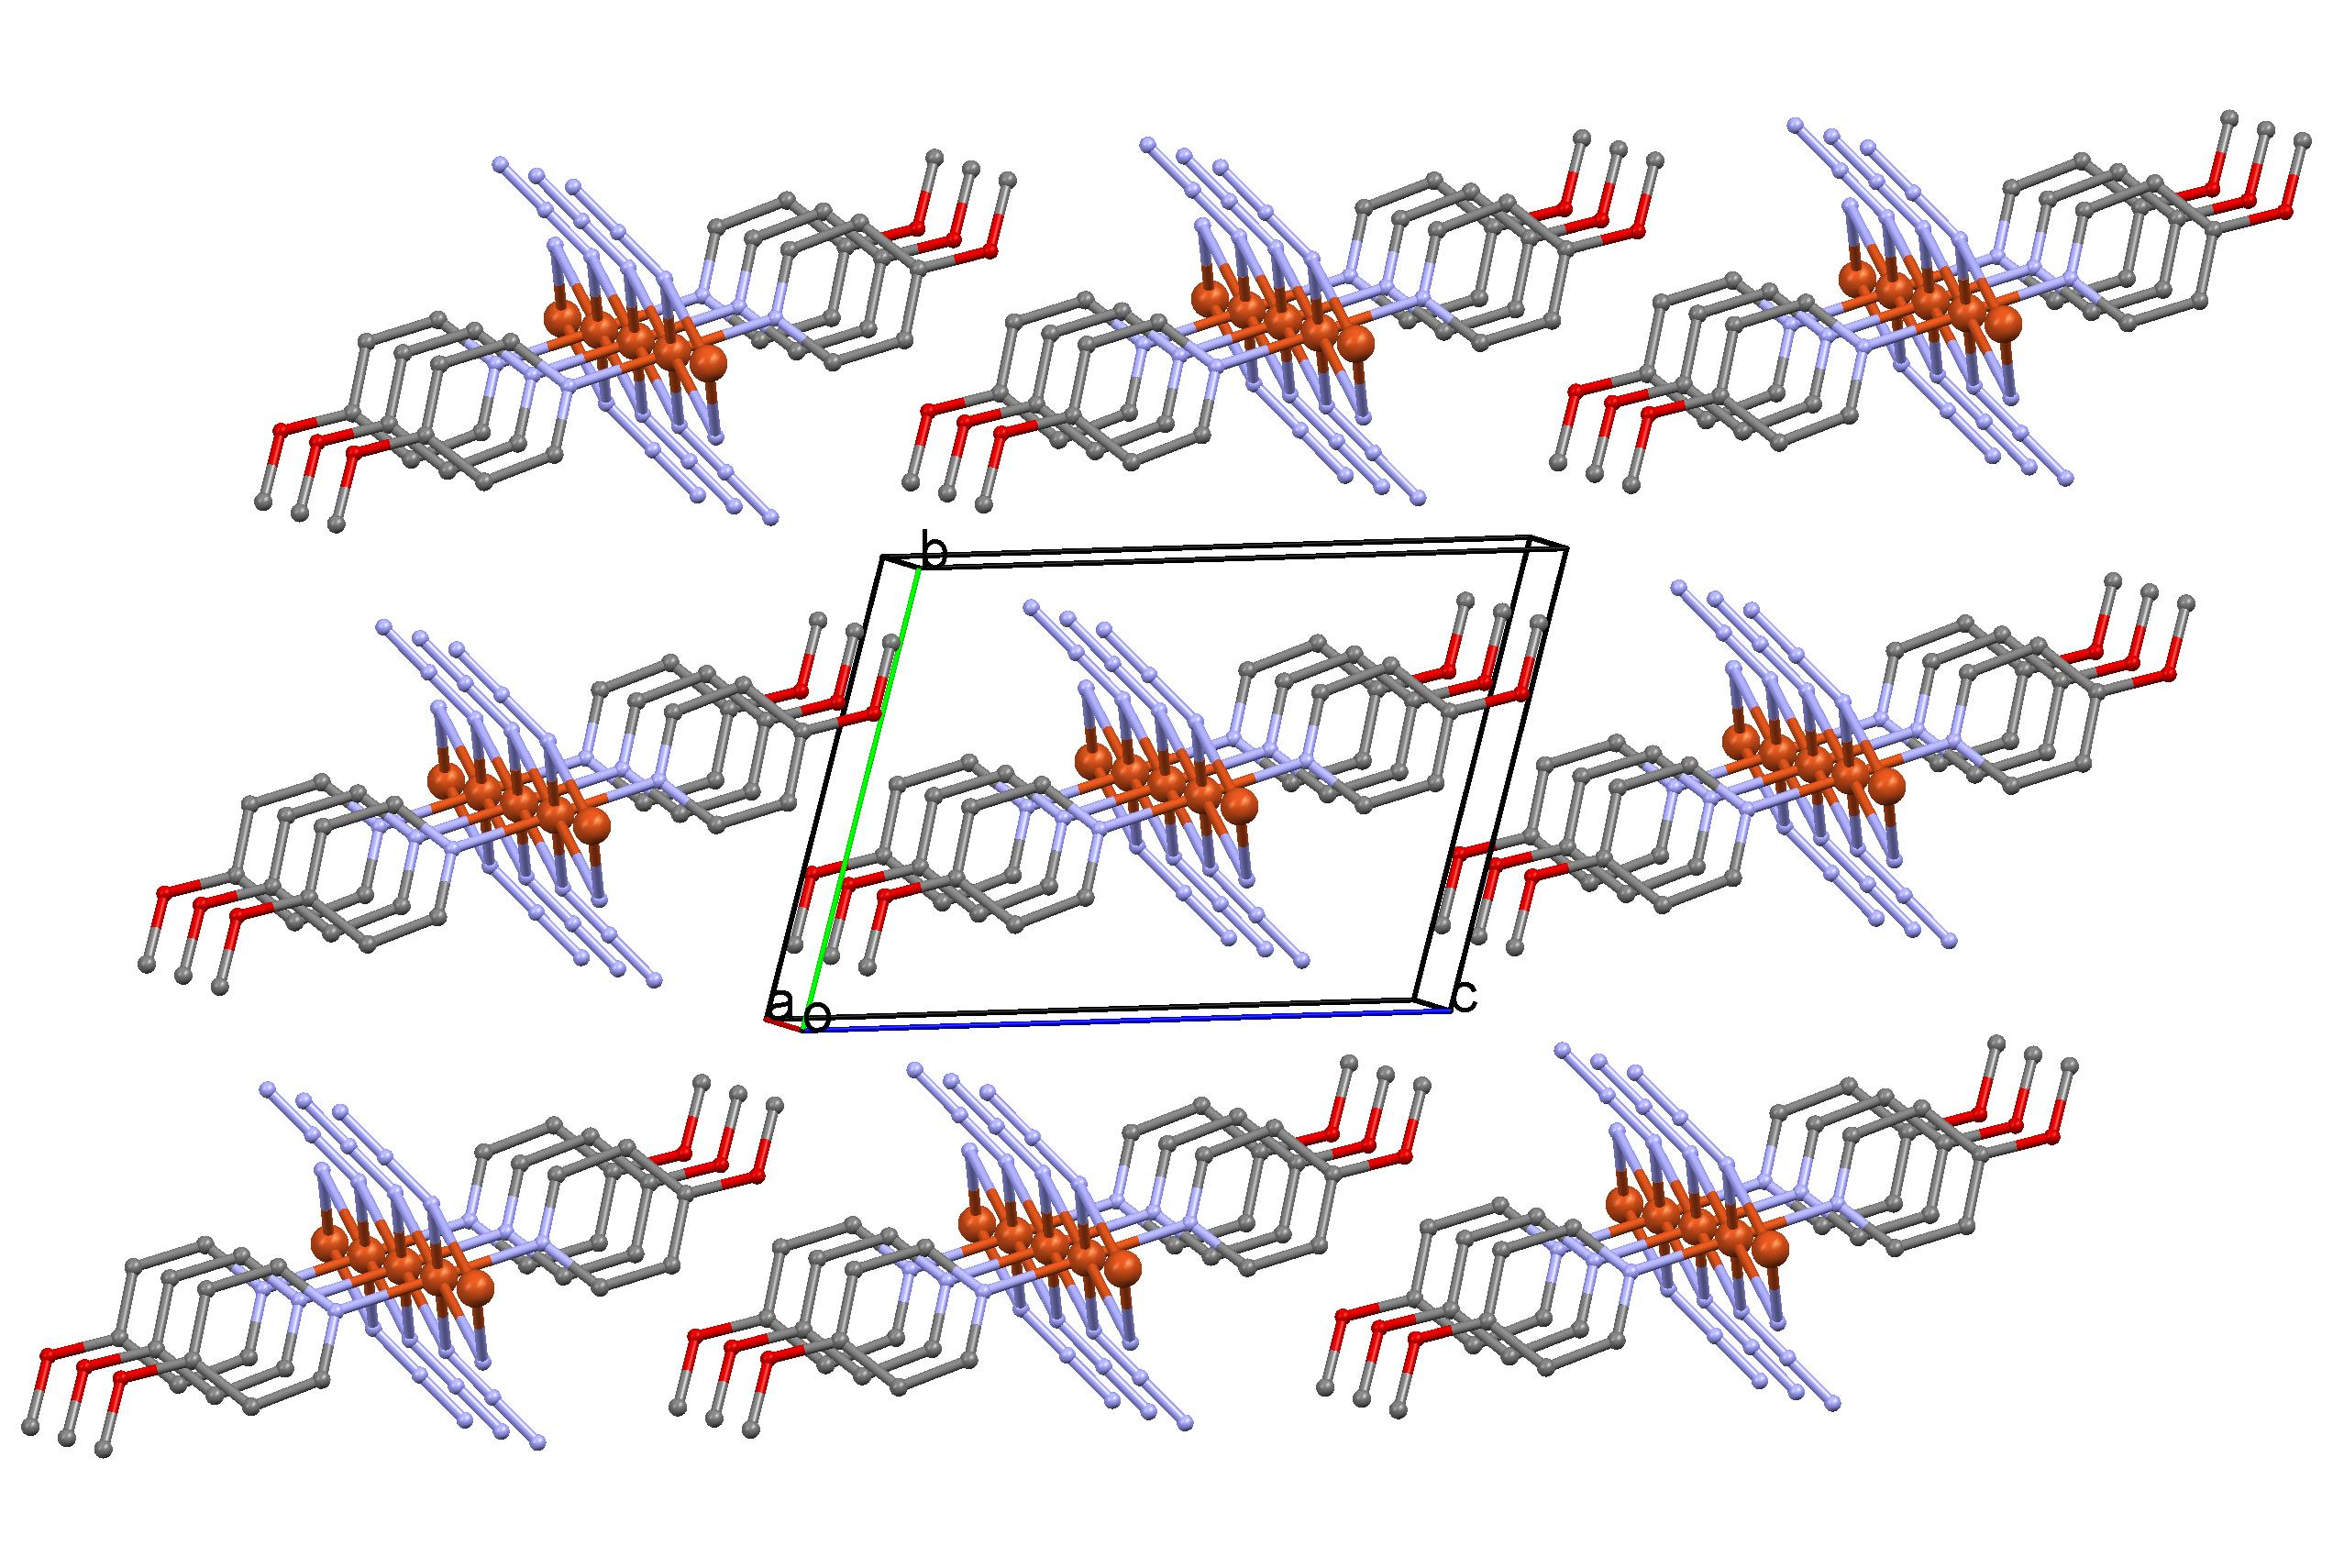
\includegraphics[width=0.95\textwidth]{figures/CuA4MOP_CA.png}
\caption{Packing plot  of \ce{[Cu(N_3)_2(4-MeOpy)_2]_n}.}
\label{fig:CuA4MOP_packv}
\end{figure}


\begin{table}
\centering
\captionabove{Crystallographic data and processing parameter of \ce{[Cu(N_3)_2(4-MeOpy)_2]_n}}
\begin{tabular}{ | l |  l | }
\hline
Empirical formula & \ce{C_{12}H_{14}CuN_{8}O_{2}}\\
\hline
Formula mass & 365.86\\
\hline
System & triclinic\\
\hline
Space group & P-1\\
\hline
a ({\AA}) & 3.6846(11)\\
\hline
b ({\AA}) & 8.755(3)\\
\hline
c ({\AA}) & 12.244(4)\\
\hline
$\alpha$ ($^\circ$) & 73.020(14)\\
\hline
$\beta$ ($^\circ$) & 85.062(16)\\
\hline
$\gamma$ ($^\circ$) & 83.034(16)\\
\hline
V (\AA$^{3}) $  & 374.4(2)\\
\hline
Z & 1\\
\hline
T (K) & 100(2)\\
\hline
$\mu$ (mm$^{-1}$) & 1.482\\
\hline
 D$_{calc}$ (Mg/m$^{3}$) & 1.623\\
\hline
Crystal size (mm) & 0.32 x 0.15 x 0.09\\
\hline
$\theta$ max ($^\circ$) & 26.98\\
\hline
Data collected & 10906\\
\hline
Unique refl./ R$_{int}$ & 1602 / 0.1163\\
\hline
Parameters & 107\\
\hline
Goodness-of-Fit on F$^{2}$ & 1.149\\
\hline
R1 / wR2 (all data) & 0.0668 /0.1567\\
\hline
Residual extrema (e/\AA$^{3}$) & 1.39 /-1.74\\
\hline
\end{tabular}

\label{ptab:CuA4MOP}

\end{table}


